\documentclass[twoside]{book}

% Packages required by doxygen
\usepackage{fixltx2e}
\usepackage{calc}
\usepackage{doxygen}
\usepackage[export]{adjustbox} % also loads graphicx
\usepackage{graphicx}
\usepackage[utf8]{inputenc}
\usepackage{makeidx}
\usepackage{multicol}
\usepackage{multirow}
\PassOptionsToPackage{warn}{textcomp}
\usepackage{textcomp}
\usepackage[nointegrals]{wasysym}
\usepackage[table]{xcolor}

% Font selection
\usepackage[T1]{fontenc}
\usepackage[scaled=.90]{helvet}
\usepackage{courier}
\usepackage{amssymb}
\usepackage{sectsty}
\renewcommand{\familydefault}{\sfdefault}
\allsectionsfont{%
  \fontseries{bc}\selectfont%
  \color{darkgray}%
}
\renewcommand{\DoxyLabelFont}{%
  \fontseries{bc}\selectfont%
  \color{darkgray}%
}
\newcommand{\+}{\discretionary{\mbox{\scriptsize$\hookleftarrow$}}{}{}}

% Page & text layout
\usepackage{geometry}
\geometry{%
  a4paper,%
  top=2.5cm,%
  bottom=2.5cm,%
  left=2.5cm,%
  right=2.5cm%
}
\tolerance=750
\hfuzz=15pt
\hbadness=750
\setlength{\emergencystretch}{15pt}
\setlength{\parindent}{0cm}
\setlength{\parskip}{0.2cm}
\makeatletter
\renewcommand{\paragraph}{%
  \@startsection{paragraph}{4}{0ex}{-1.0ex}{1.0ex}{%
    \normalfont\normalsize\bfseries\SS@parafont%
  }%
}
\renewcommand{\subparagraph}{%
  \@startsection{subparagraph}{5}{0ex}{-1.0ex}{1.0ex}{%
    \normalfont\normalsize\bfseries\SS@subparafont%
  }%
}
\makeatother

% Headers & footers
\usepackage{fancyhdr}
\pagestyle{fancyplain}
\fancyhead[LE]{\fancyplain{}{\bfseries\thepage}}
\fancyhead[CE]{\fancyplain{}{}}
\fancyhead[RE]{\fancyplain{}{\bfseries\leftmark}}
\fancyhead[LO]{\fancyplain{}{\bfseries\rightmark}}
\fancyhead[CO]{\fancyplain{}{}}
\fancyhead[RO]{\fancyplain{}{\bfseries\thepage}}
\fancyfoot[LE]{\fancyplain{}{}}
\fancyfoot[CE]{\fancyplain{}{}}
\fancyfoot[RE]{\fancyplain{}{\bfseries\scriptsize Generated on Mon Nov 16 2015 18\+:31\+:54 for My Project by Doxygen }}
\fancyfoot[LO]{\fancyplain{}{\bfseries\scriptsize Generated on Mon Nov 16 2015 18\+:31\+:54 for My Project by Doxygen }}
\fancyfoot[CO]{\fancyplain{}{}}
\fancyfoot[RO]{\fancyplain{}{}}
\renewcommand{\footrulewidth}{0.4pt}
\renewcommand{\chaptermark}[1]{%
  \markboth{#1}{}%
}
\renewcommand{\sectionmark}[1]{%
  \markright{\thesection\ #1}%
}

% Indices & bibliography
\usepackage{natbib}
\usepackage[titles]{tocloft}
\setcounter{tocdepth}{3}
\setcounter{secnumdepth}{5}
\makeindex

% Hyperlinks (required, but should be loaded last)
\usepackage{ifpdf}
\ifpdf
  \usepackage[pdftex,pagebackref=true]{hyperref}
\else
  \usepackage[ps2pdf,pagebackref=true]{hyperref}
\fi
\hypersetup{%
  colorlinks=true,%
  linkcolor=blue,%
  citecolor=blue,%
  unicode%
}

% Custom commands
\newcommand{\clearemptydoublepage}{%
  \newpage{\pagestyle{empty}\cleardoublepage}%
}


%===== C O N T E N T S =====

\begin{document}

% Titlepage & ToC
\hypersetup{pageanchor=false,
             bookmarks=true,
             bookmarksnumbered=true,
             pdfencoding=unicode
            }
\pagenumbering{roman}
\begin{titlepage}
\vspace*{7cm}
\begin{center}%
{\Large My Project }\\
\vspace*{1cm}
{\large Generated by Doxygen 1.8.10}\\
\vspace*{0.5cm}
{\small Mon Nov 16 2015 18:31:54}\\
\end{center}
\end{titlepage}
\clearemptydoublepage
\tableofcontents
\clearemptydoublepage
\pagenumbering{arabic}
\hypersetup{pageanchor=true}

%--- Begin generated contents ---
\chapter{S\+E\+N\+G330\+\_\+\+Assign2}
\label{md__r_e_a_d_m_e}
\hypertarget{md__r_e_a_d_m_e}{}
Assignment 2 for S\+E\+N\+G 330, writing Prototype Design Pattern example in C++ and creating framework 
\chapter{Hierarchical Index}
\section{Class Hierarchy}
This inheritance list is sorted roughly, but not completely, alphabetically\+:\begin{DoxyCompactList}
\item \contentsline{section}{Gym\+Machine}{\pageref{class_gym_machine}}{}
\begin{DoxyCompactList}
\item \contentsline{section}{Rowing\+Machine}{\pageref{class_rowing_machine}}{}
\item \contentsline{section}{Treadmill}{\pageref{class_treadmill}}{}
\end{DoxyCompactList}
\end{DoxyCompactList}

\chapter{Class Index}
\section{Class List}
Here are the classes, structs, unions and interfaces with brief descriptions\+:\begin{DoxyCompactList}
\item\contentsline{section}{\hyperlink{class_gym_machine}{Gym\+Machine} \\*Super Class \hyperlink{class_gym_machine}{Gym\+Machine} }{\pageref{class_gym_machine}}{}
\item\contentsline{section}{\hyperlink{class_rowing_machine}{Rowing\+Machine} \\*Sub Class \hyperlink{class_rowing_machine}{Rowing\+Machine} }{\pageref{class_rowing_machine}}{}
\item\contentsline{section}{\hyperlink{class_treadmill}{Treadmill} \\*Sub Class \hyperlink{class_treadmill}{Treadmill} }{\pageref{class_treadmill}}{}
\end{DoxyCompactList}

\chapter{Class Documentation}
\hypertarget{class_gym_machine}{}\section{Gym\+Machine Class Reference}
\label{class_gym_machine}\index{Gym\+Machine@{Gym\+Machine}}


Super Class \hyperlink{class_gym_machine}{Gym\+Machine}.  


Inheritance diagram for Gym\+Machine\+:\begin{figure}[H]
\begin{center}
\leavevmode
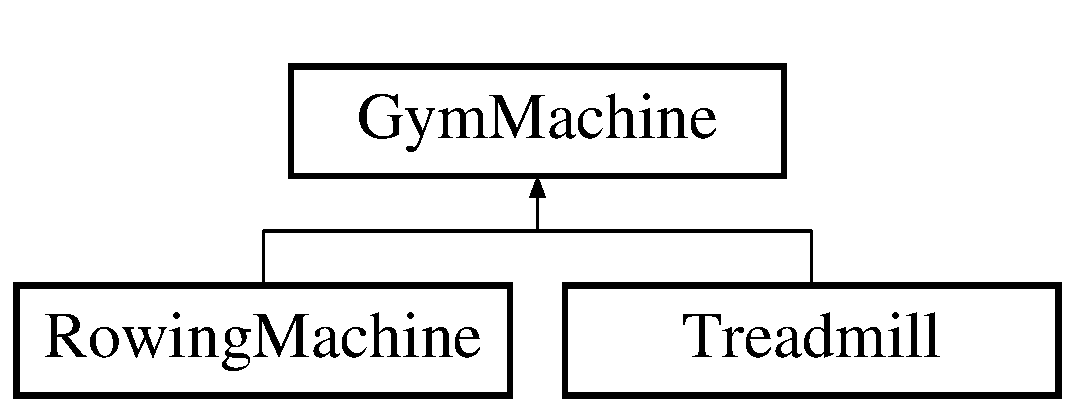
\includegraphics[height=2.000000cm]{class_gym_machine}
\end{center}
\end{figure}
\subsection*{Public Member Functions}
\begin{DoxyCompactItemize}
\item 
\hypertarget{class_gym_machine_a85345b529a91c02b60ccb43bf9d554a4}{}\hyperlink{class_gym_machine_a85345b529a91c02b60ccb43bf9d554a4}{Gym\+Machine} (int power, int area)\label{class_gym_machine_a85345b529a91c02b60ccb43bf9d554a4}

\begin{DoxyCompactList}\small\item\em Constructor for \hyperlink{class_gym_machine}{Gym\+Machine}, takes both power and size parameters. \end{DoxyCompactList}\item 
\hypertarget{class_gym_machine_a80c7858fd921a01e91457dc1fb3383ad}{}\hyperlink{class_gym_machine_a80c7858fd921a01e91457dc1fb3383ad}{Gym\+Machine} (const \hyperlink{class_gym_machine}{Gym\+Machine} $\ast$other)\label{class_gym_machine_a80c7858fd921a01e91457dc1fb3383ad}

\begin{DoxyCompactList}\small\item\em Copy Constructor for \hyperlink{class_gym_machine}{Gym\+Machine}, takes pointer to a \hyperlink{class_gym_machine}{Gym\+Machine} as a parameter to copy. \end{DoxyCompactList}\end{DoxyCompactItemize}
\subsection*{Public Attributes}
\begin{DoxyCompactItemize}
\item 
\hypertarget{class_gym_machine_a680693dad7672fe9917de8951f59d182}{}int \hyperlink{class_gym_machine_a680693dad7672fe9917de8951f59d182}{power\+Consumption}\label{class_gym_machine_a680693dad7672fe9917de8951f59d182}

\begin{DoxyCompactList}\small\item\em Amount of power a particular machine will consume. \end{DoxyCompactList}\item 
\hypertarget{class_gym_machine_aa9dca285aa8e1fc53eb252cb691d3a69}{}int \hyperlink{class_gym_machine_aa9dca285aa8e1fc53eb252cb691d3a69}{size}\label{class_gym_machine_aa9dca285aa8e1fc53eb252cb691d3a69}

\begin{DoxyCompactList}\small\item\em The size of the machine in square feet. \end{DoxyCompactList}\end{DoxyCompactItemize}


\subsection{Detailed Description}
Super Class \hyperlink{class_gym_machine}{Gym\+Machine}. 

\hyperlink{class_gym_machine}{Gym\+Machine} is the super class to all the different classes representing machines within a gym, in this current case just Treadmills and Rowing Machines.

\hyperlink{class_gym_machine}{Gym\+Machine} holds both the amount of power consumed by the machine and the size of the machine as both of these variables apply to all machines in this scenario(all machines will theoretically communicate with a central system even something possibly non-\/electric like a rowing machine will still consume power for the onboard computer) 

The documentation for this class was generated from the following file\+:\begin{DoxyCompactItemize}
\item 
assign2\+\_\+gym.\+cpp\end{DoxyCompactItemize}

\hypertarget{class_rowing_machine}{}\section{Rowing\+Machine Class Reference}
\label{class_rowing_machine}\index{Rowing\+Machine@{Rowing\+Machine}}


Sub Class \hyperlink{class_rowing_machine}{Rowing\+Machine}.  


Inheritance diagram for Rowing\+Machine\+:\begin{figure}[H]
\begin{center}
\leavevmode
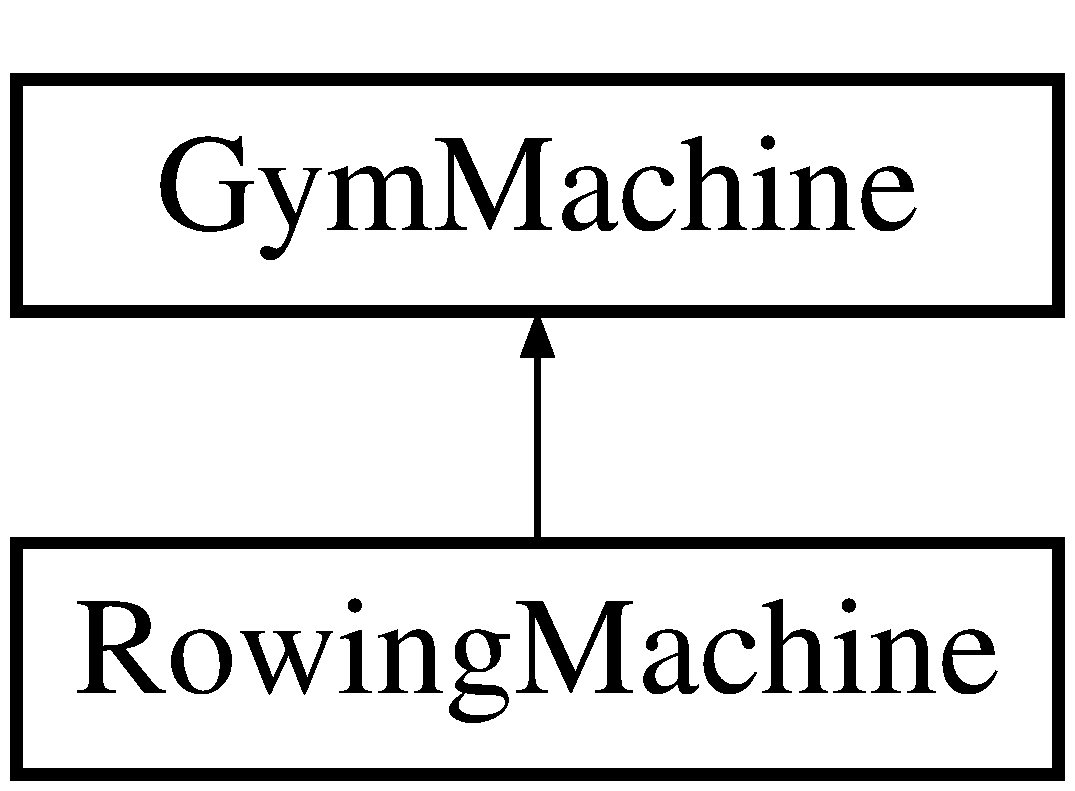
\includegraphics[height=2.000000cm]{class_rowing_machine}
\end{center}
\end{figure}
\subsection*{Public Member Functions}
\begin{DoxyCompactItemize}
\item 
\hypertarget{class_rowing_machine_a93540e47856483f363f7479bde8990e4}{}\hyperlink{class_rowing_machine_a93540e47856483f363f7479bde8990e4}{Rowing\+Machine} (int resist)\label{class_rowing_machine_a93540e47856483f363f7479bde8990e4}

\begin{DoxyCompactList}\small\item\em Constructor for \hyperlink{class_rowing_machine}{Rowing\+Machine}, since it inherits from \hyperlink{class_gym_machine}{Gym\+Machine} it passes in default values of 25 and 7 for power and size to the super class constructor. \end{DoxyCompactList}\item 
\hypertarget{class_rowing_machine_a53fae8a736890b349d9fee54c11dd182}{}\hyperlink{class_rowing_machine_a53fae8a736890b349d9fee54c11dd182}{Rowing\+Machine} (const \hyperlink{class_rowing_machine}{Rowing\+Machine} $\ast$other)\label{class_rowing_machine_a53fae8a736890b349d9fee54c11dd182}

\begin{DoxyCompactList}\small\item\em Copy Constructor for \hyperlink{class_rowing_machine}{Rowing\+Machine}, calls the copy constructor of \hyperlink{class_gym_machine}{Gym\+Machine} to complete the copy. \end{DoxyCompactList}\item 
\hypertarget{class_rowing_machine_a494a8b0cc7a5ada40cb9cce3f1f8a2eb}{}\hyperlink{class_rowing_machine}{Rowing\+Machine} $\ast$ \hyperlink{class_rowing_machine_a494a8b0cc7a5ada40cb9cce3f1f8a2eb}{clone} (int resist)\label{class_rowing_machine_a494a8b0cc7a5ada40cb9cce3f1f8a2eb}

\begin{DoxyCompactList}\small\item\em Clone function used as part of Prototype design pattern, returns a new \hyperlink{class_rowing_machine}{Rowing\+Machine} based off the prototype \textquotesingle{}row\textquotesingle{}. \end{DoxyCompactList}\end{DoxyCompactItemize}
\subsection*{Public Attributes}
\begin{DoxyCompactItemize}
\item 
\hypertarget{class_rowing_machine_a3c5f0c2e988e3e92cca2a02efb73d7fc}{}int \hyperlink{class_rowing_machine_a3c5f0c2e988e3e92cca2a02efb73d7fc}{resistance}\label{class_rowing_machine_a3c5f0c2e988e3e92cca2a02efb73d7fc}

\begin{DoxyCompactList}\small\item\em The amount of resistance to pulling the handle of the Rowing Machine. \end{DoxyCompactList}\end{DoxyCompactItemize}


\subsection{Detailed Description}
Sub Class \hyperlink{class_rowing_machine}{Rowing\+Machine}. 

\hyperlink{class_rowing_machine}{Rowing\+Machine} is a sub class of \hyperlink{class_gym_machine}{Gym\+Machine}

\hyperlink{class_rowing_machine}{Rowing\+Machine}\textquotesingle{}s have one unique variable which is the resistance set for the machine \hyperlink{class_rowing_machine}{Rowing\+Machine}\textquotesingle{}s also work with the Prototype design pattern, so a clone function is used to create a new instance of the class based off of the pre-\/existing prototype referred to as \textquotesingle{}row\textquotesingle{} 

The documentation for this class was generated from the following file\+:\begin{DoxyCompactItemize}
\item 
assign2\+\_\+gym.\+cpp\end{DoxyCompactItemize}

\hypertarget{class_treadmill}{}\section{Treadmill Class Reference}
\label{class_treadmill}\index{Treadmill@{Treadmill}}


Sub Class \hyperlink{class_treadmill}{Treadmill}.  


Inheritance diagram for Treadmill\+:\begin{figure}[H]
\begin{center}
\leavevmode
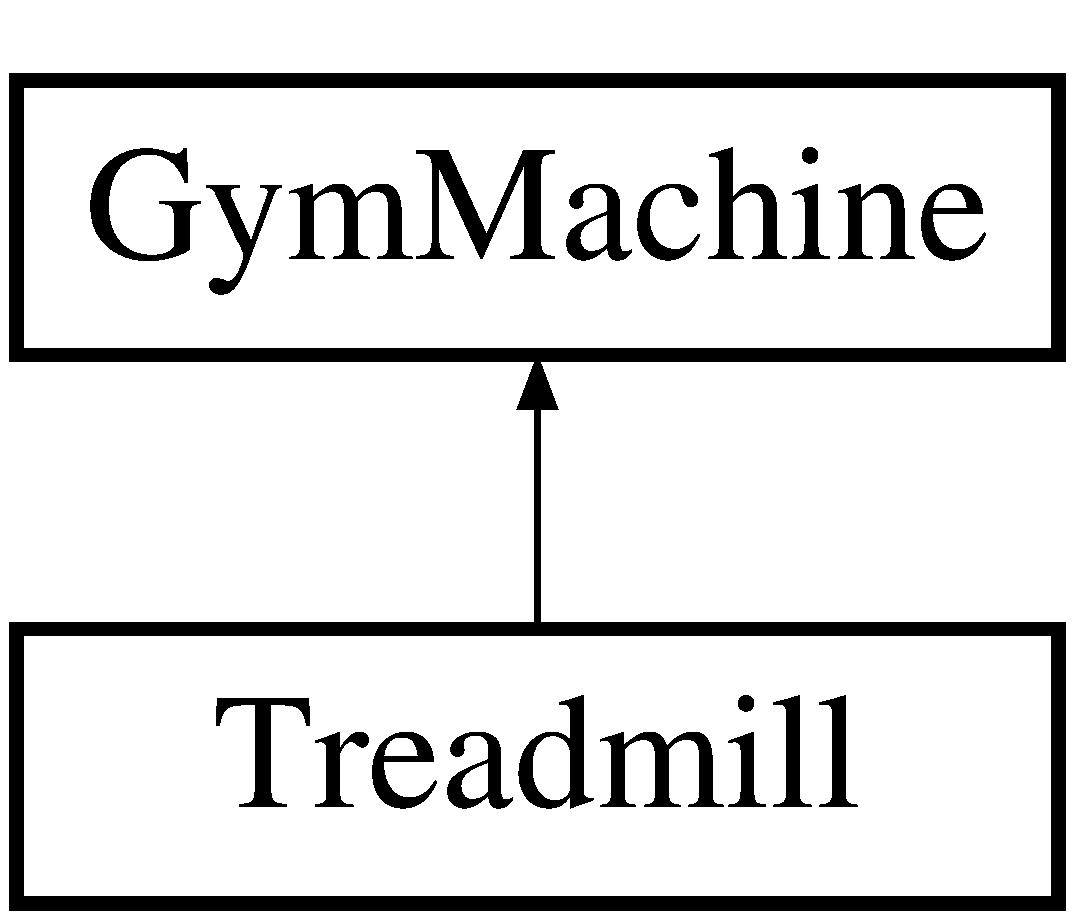
\includegraphics[height=2.000000cm]{class_treadmill}
\end{center}
\end{figure}
\subsection*{Public Member Functions}
\begin{DoxyCompactItemize}
\item 
\hypertarget{class_treadmill_a729fe8dba8c5be57f4b74de245b409f4}{}\hyperlink{class_treadmill_a729fe8dba8c5be57f4b74de245b409f4}{Treadmill} (int speed)\label{class_treadmill_a729fe8dba8c5be57f4b74de245b409f4}

\begin{DoxyCompactList}\small\item\em Constructor for \hyperlink{class_treadmill}{Treadmill}, since it inherits from \hyperlink{class_gym_machine}{Gym\+Machine} it passes in default values of 10 and 5 for power and size to the super class constructor. \end{DoxyCompactList}\item 
\hypertarget{class_treadmill_a6061b1313ceddd6f631fcd9bc7999afd}{}\hyperlink{class_treadmill_a6061b1313ceddd6f631fcd9bc7999afd}{Treadmill} (const \hyperlink{class_treadmill}{Treadmill} $\ast$other)\label{class_treadmill_a6061b1313ceddd6f631fcd9bc7999afd}

\begin{DoxyCompactList}\small\item\em Copy Constructor for \hyperlink{class_treadmill}{Treadmill}, uses copy constructor of \hyperlink{class_gym_machine}{Gym\+Machine}. \end{DoxyCompactList}\item 
\hypertarget{class_treadmill_ab855c0fb00dda980bb02111caf3416de}{}\hyperlink{class_treadmill}{Treadmill} $\ast$ \hyperlink{class_treadmill_ab855c0fb00dda980bb02111caf3416de}{clone} (int speed)\label{class_treadmill_ab855c0fb00dda980bb02111caf3416de}

\begin{DoxyCompactList}\small\item\em clone function used in Prototype design pattern, creates new \hyperlink{class_treadmill}{Treadmill} from prototype \textquotesingle{}tread\textquotesingle{} \end{DoxyCompactList}\end{DoxyCompactItemize}
\subsection*{Public Attributes}
\begin{DoxyCompactItemize}
\item 
\hypertarget{class_treadmill_a11186946bfc29bc3dc83aaf11fd5f22f}{}int \hyperlink{class_treadmill_a11186946bfc29bc3dc83aaf11fd5f22f}{max\+Speed}\label{class_treadmill_a11186946bfc29bc3dc83aaf11fd5f22f}

\begin{DoxyCompactList}\small\item\em The max speed that the spinning belt of the \hyperlink{class_treadmill}{Treadmill} can run at. \end{DoxyCompactList}\end{DoxyCompactItemize}


\subsection{Detailed Description}
Sub Class \hyperlink{class_treadmill}{Treadmill}. 

\hyperlink{class_treadmill}{Treadmill} is a sub class of \hyperlink{class_gym_machine}{Gym\+Machine}

\hyperlink{class_treadmill}{Treadmill}\textquotesingle{}s have one unique variable which is their maximum speed for the belt \hyperlink{class_treadmill}{Treadmill}\textquotesingle{}s also work with the Prototype design pattern, so a clone function is used to create a new instance of the class based off of the pre-\/existing prototype referred to as \textquotesingle{}tread\textquotesingle{} 

The documentation for this class was generated from the following file\+:\begin{DoxyCompactItemize}
\item 
assign2\+\_\+gym.\+cpp\end{DoxyCompactItemize}

%--- End generated contents ---

% Index
\backmatter
\newpage
\phantomsection
\clearemptydoublepage
\addcontentsline{toc}{chapter}{Index}
\printindex

\end{document}
